%\section{Study of tau lepton in truth level} 
%\label{app:truth_tau}

In addition to selecting the four-lepton events with `lepton' only including electron and muon ($4e$, $2e2\mu$ and $4\mu$ channels), 
a serious studies of considering $2e2\tau$ and $2\mu2\tau$ channels in final states have been done in particle-level.
Without considering fake background and the rather complicated decay results of $\tau$-lepton, the study in particle-level is a good start point.

The object selections of electron and muon and the event level selections for leptons (now including $\tau$) are still keep the same as described in previous two sections.
For the selection of $\tau$-lepton: it must satisfy $\pt > 20~\gev$ and be measured in the pseudorapidity range of $\left|\eta \right|<2.5$.
And to minic the reconstruction performance, for all leptons, a flat reconstruction efficiency is applied in object selection of electron, muon and $\tau$-lepton.
A $85\%~(95\%)$ efficiency is applied to electron (muon),
while to hadronic decay $\tau$, the reconstruction efficiency of 50\% times its hadronic decay rate is signed. 
And for its leptonic decay, the efficiency is the same as the one to electron and muon. 
In summary, the overall reconstruction efficiency to $\tau$-lepton is about 64\%.

\textbf{Considering only the visible decay product for the reconstruction of $\tau$-lepton}

%To be more closed to reconstruction level measurement, we ues only the reconstructed 
%visible part of tau in truth level which not include those neutrinos from tau decay.
Figure~\ref{fig:Ztt_mass} shows the invariant mass distribution of Z bosons reconstructed from two $\tau$s using three different kinds of $\tau$-lepton:
\begin{itemize}
	\item The $\tau$-lepton is reconstructed from both visible decay product (eg. electrons, muons, hardons) and the invisible neutrinos (can be extracted in particle-level from decay chain).
	\item In addition to the previous case, the energy of photon from decay product is also added, which is called `dressing' in particle-level.
	\item Only consider the visible part from $\tau$-lepton decay, as in reconstruction-level, the decay product of neutrinos are hard to be reconstructed.
\end{itemize} 
Clear energy loss is seen for the thrid case with only visible $\tau$ decay product in Figure~\ref{fig:Ztt_mass}.
\begin{figure}[!htbp]
\centering
\subfloat[]{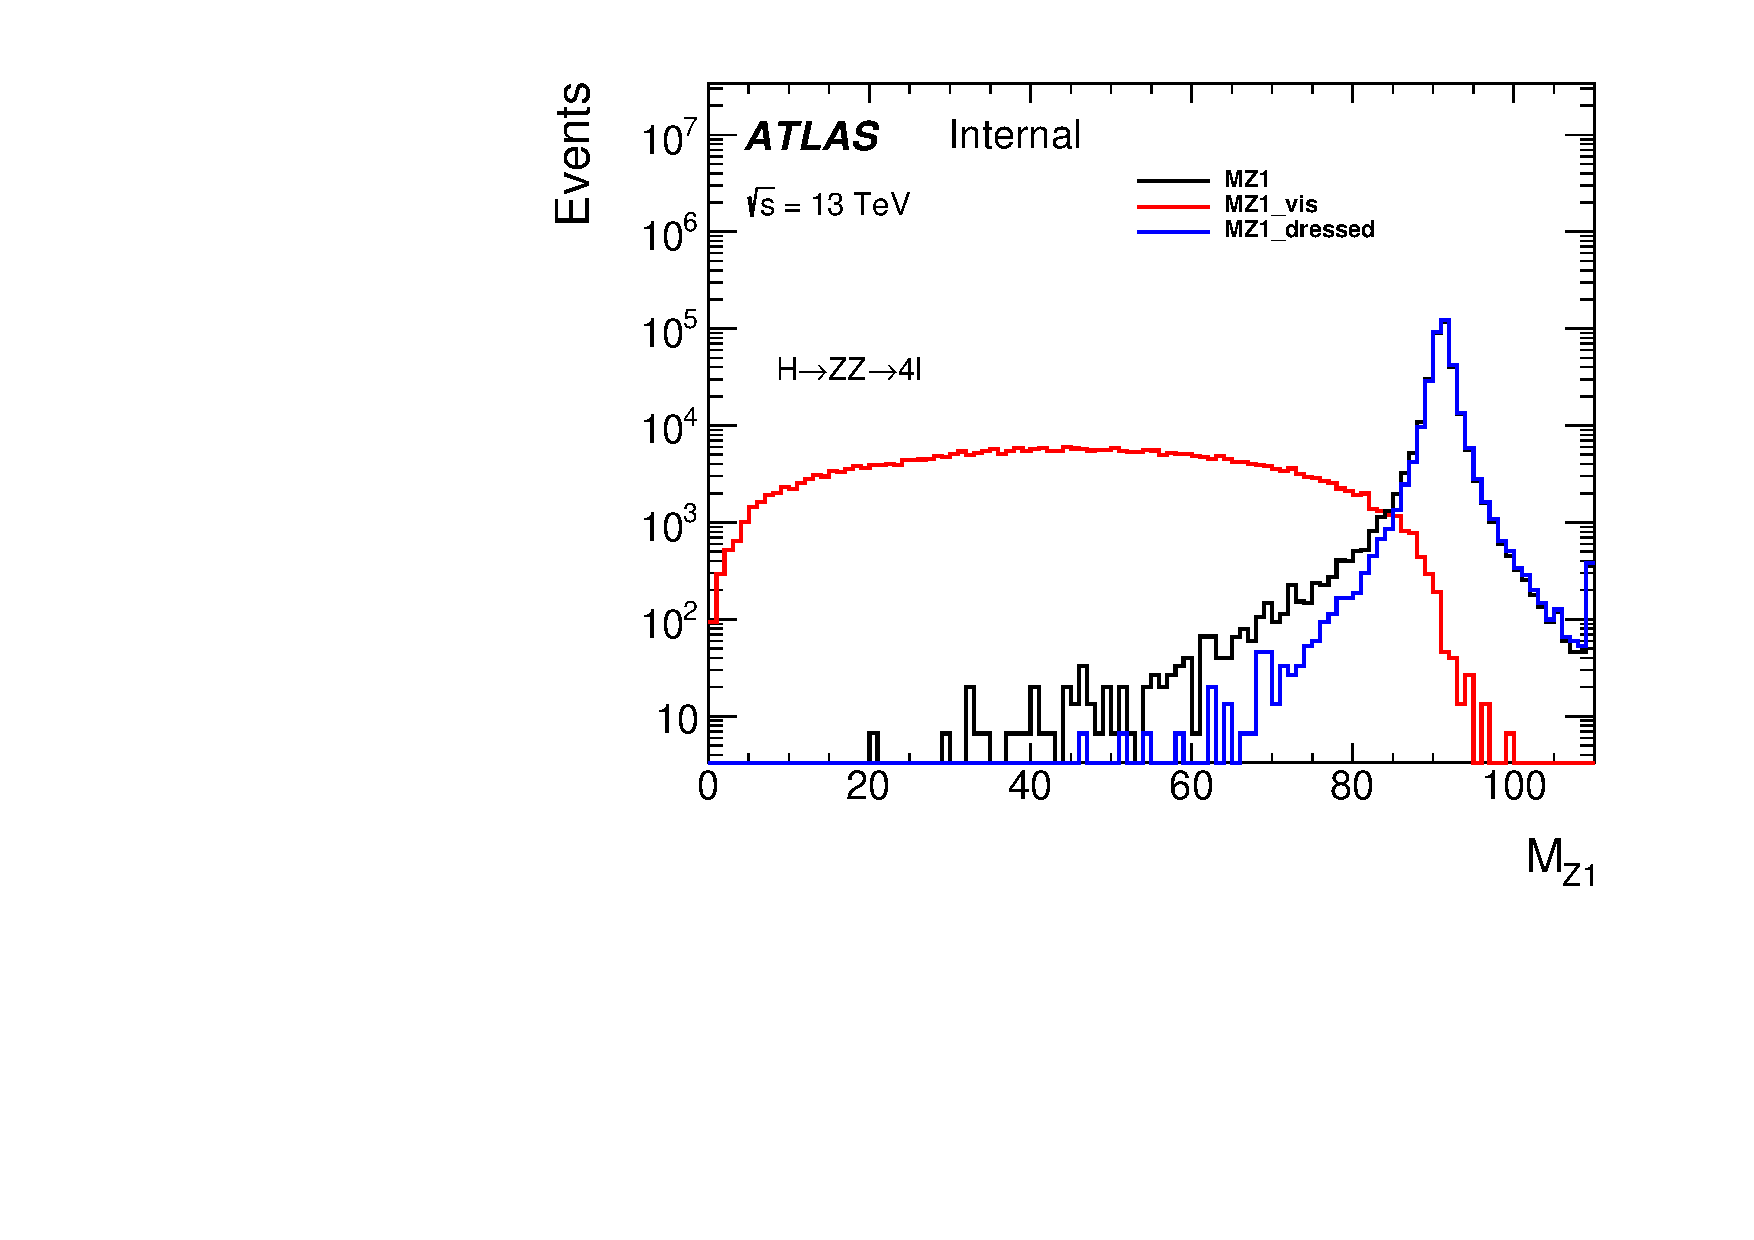
\includegraphics[width=0.48\textwidth]{figures/HMHZZ/truthTau/MZ1_comp_300NW_log.pdf}}
\subfloat[]{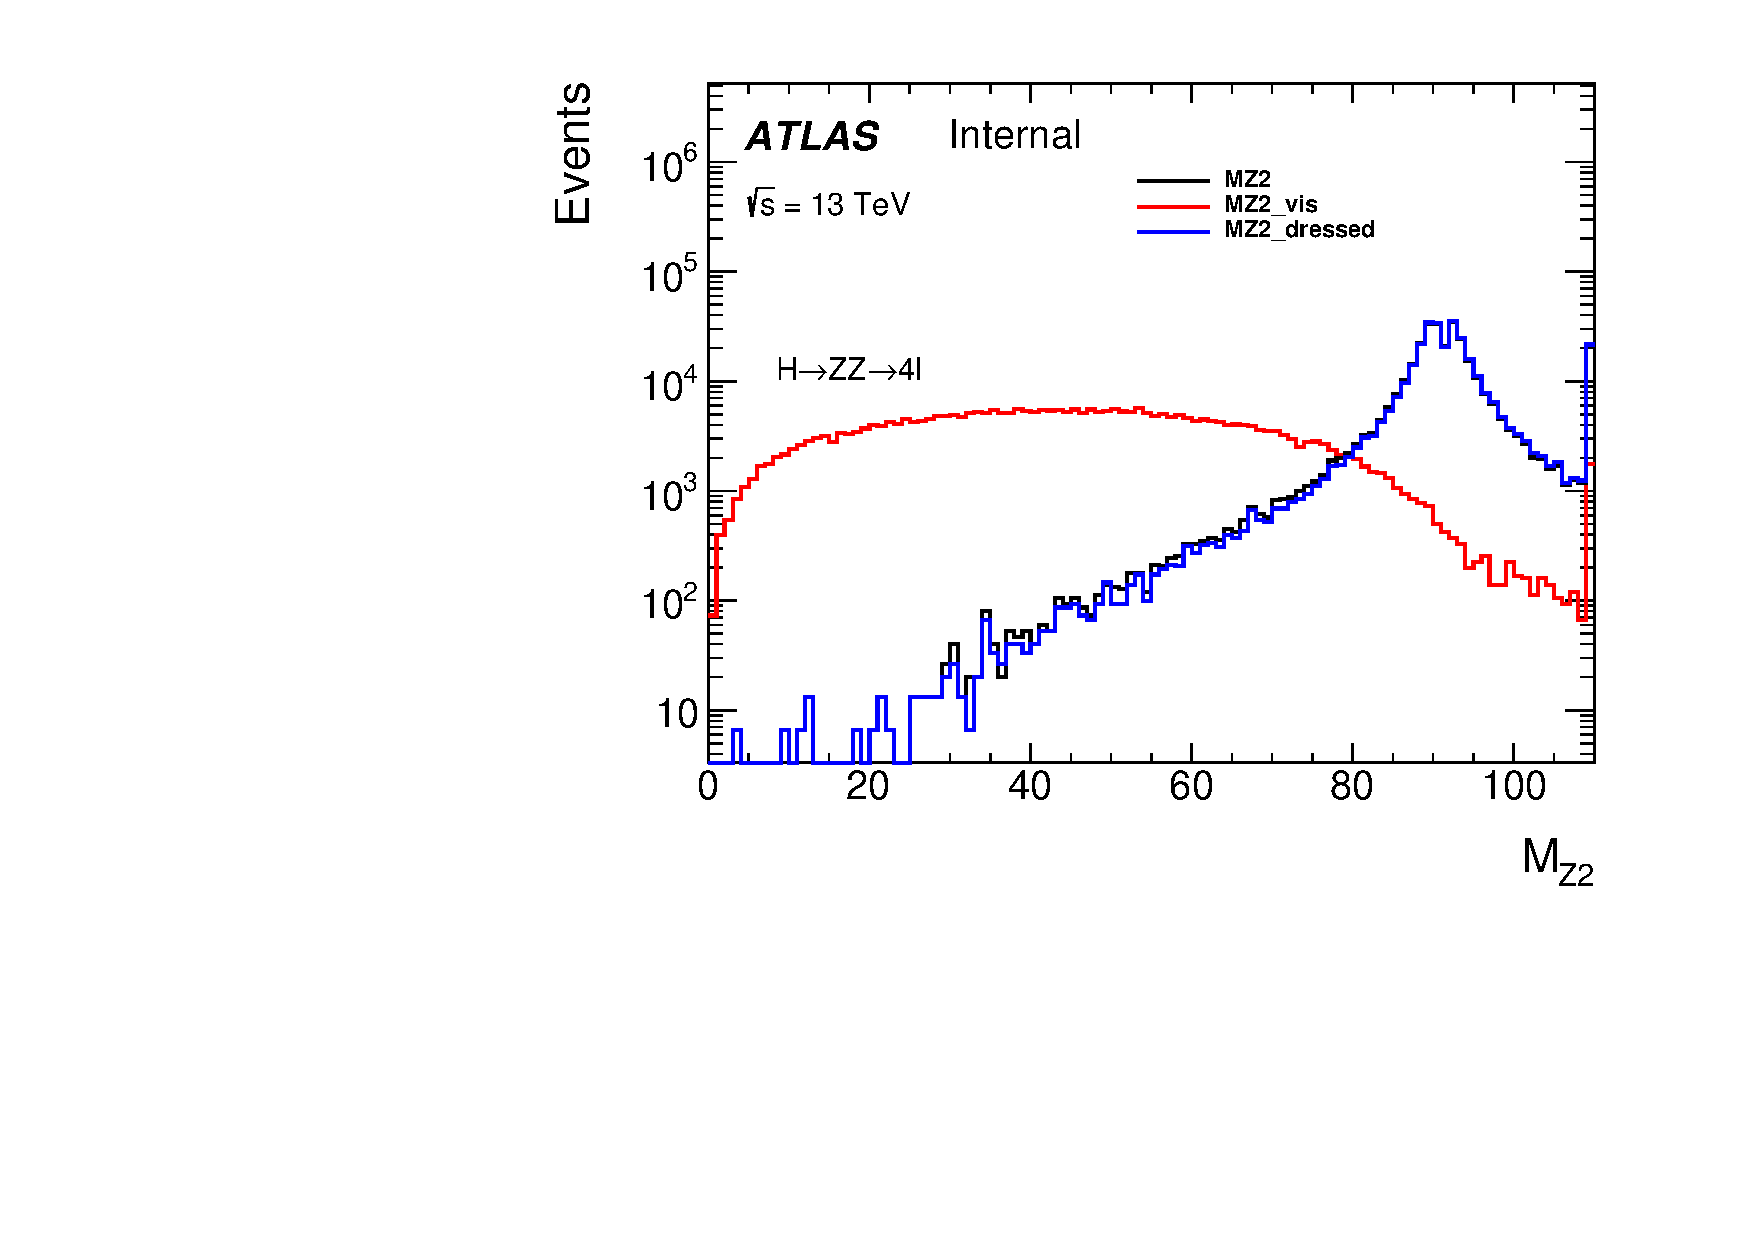
\includegraphics[width=0.48\textwidth]{figures/HMHZZ/truthTau/MZ2_comp_300NW_log.pdf}}
\caption{
Z(\rightarrow $\tau\tau$) boson invairant mass distribution for signal at 300~\gev~of
(a) $M_{Z1}$: the leading pairs;
(b) $M_{Z2}$: the sub-leading pairs.
The defination of leading and sub-leading pairs can be found in section~\ref{sec:hmhzz_eventsel}.
}
\label{fig:Ztt_mass}
\end{figure}

To check the performace in reconstruction-level, only the visible decay product is used for the reconstruction of $\tau$ in the following studies.
Then the expected number of events for signal and \qqZZ background in different lepton flavor channels are shown in table~\ref{tab:yield_diffMass} by normalizing to the luminosity of 80~\ifb.
Three different kind of final states are considered:
\begin{itemize}
	\item Inclusive: channels including $2e2\mu$, $4e$, $4\mu$ and $2e2\tau$, $2\mu2tau$.
	\item Only e$\mu$: $2e2\mu$, $4e$, $4\mu$ channels.
	\item With $\tau$: $2e2\tau$, $2\mu2tau$ channels.
\end{itemize}
The simulated narrow-width signal samples at the \mH of 300, 600, 1000 and 1200~\gev~ are studied.

\begin{table}[htbp]
  \centering
  \caption{The expected number of events for signal and \qqZZ background in the lepton flavor channels with or without $\tau$-lepton.
	The event yields are normalized to the luminosity of 80~\ifb.}
  \label{tab:yield_diffMass}
  \begin{tabular}{|c|c|c|c|c|c|}
    \hline
     \multirow{2}*{Mass window} & \multirow{2}*{Channels} & \multicolumn{2}{c|}{signal} & \multicolumn{2}{c|}{\qqZZ} \\
    \cline{3-6} 
      & ~ & Events & Fraction & Events & Fraction \\
    \hline
    \multirow{3}*{[250\gev, 350\gev]}  & Inclusive & 3423.5 & $100\%$  & 539.1 & $100\%$ \\
    \cline{2-6}
    ~                                  & Only e$\mu$   & 3148.2 & $92.0\%$ & 493.8 & $91.6\%$ \\
    \cline{2-6}
    ~                                  & With $\tau$  & 275.4  & $8.0\%$  & 42.7  & $7.9\%$ \\
    \hline
    \multirow{3}*{[550\gev, 650\gev]}  & Inclusive & 1312.1 & $100\%$  & 26.0 & $100\%$ \\
    \cline{2-6}
    ~                                  & Only e$\mu$   & 1269.9 & $96.8\%$ & 24.1 & $92.6\%$ \\
    \cline{2-6}
    ~                                  & With $\tau$  & 42.2   & $3.2\%$  & 1.7  & $6.5\%$ \\
    \hline
    \multirow{3}*{[950\gev, 1050\gev]} & Inclusive & 526.9 & $100\%$  & 1.20 & $100\%$ \\
    \cline{2-6}
    ~                                  & Only e$\mu$   & 529.9 & $98.7\%$ & 1.18 & $98.5\%$ \\
    \cline{2-6}
    ~                                  & With $\tau$  & 7.0   & $1.3\%$  & 0.12 & $10.4\%$ \\
    \hline
    \multirow{3}*{[1150\gev, 1350\gev]}& Inclusive & 419.1 & $100\%$  & 1.09 & $100\%$ \\
    \cline{2-6}
    ~                                  & Only e$\mu$   & 414.9 & $99.0\%$ & 1.07 & $98.7\%$ \\
    \cline{2-6}
    ~                                  & With $\tau$  & 4.1   & $1.0\%$  &  0   & $0\%$ \\
    \hline
  \end{tabular}
\end{table}

Figure~\ref{fig:tau_signif} shows the significance scan as a function of \mfl at four mass points: 300, 600, 1000, 1200~\gev, for events in lepton flavor channel with or without $\tau$-lepton. 
A profile likehood function is used for scan, and the background only considers the contribution from \qqZZ.

\begin{figure}[!htbp]
\centering
\subfloat[]{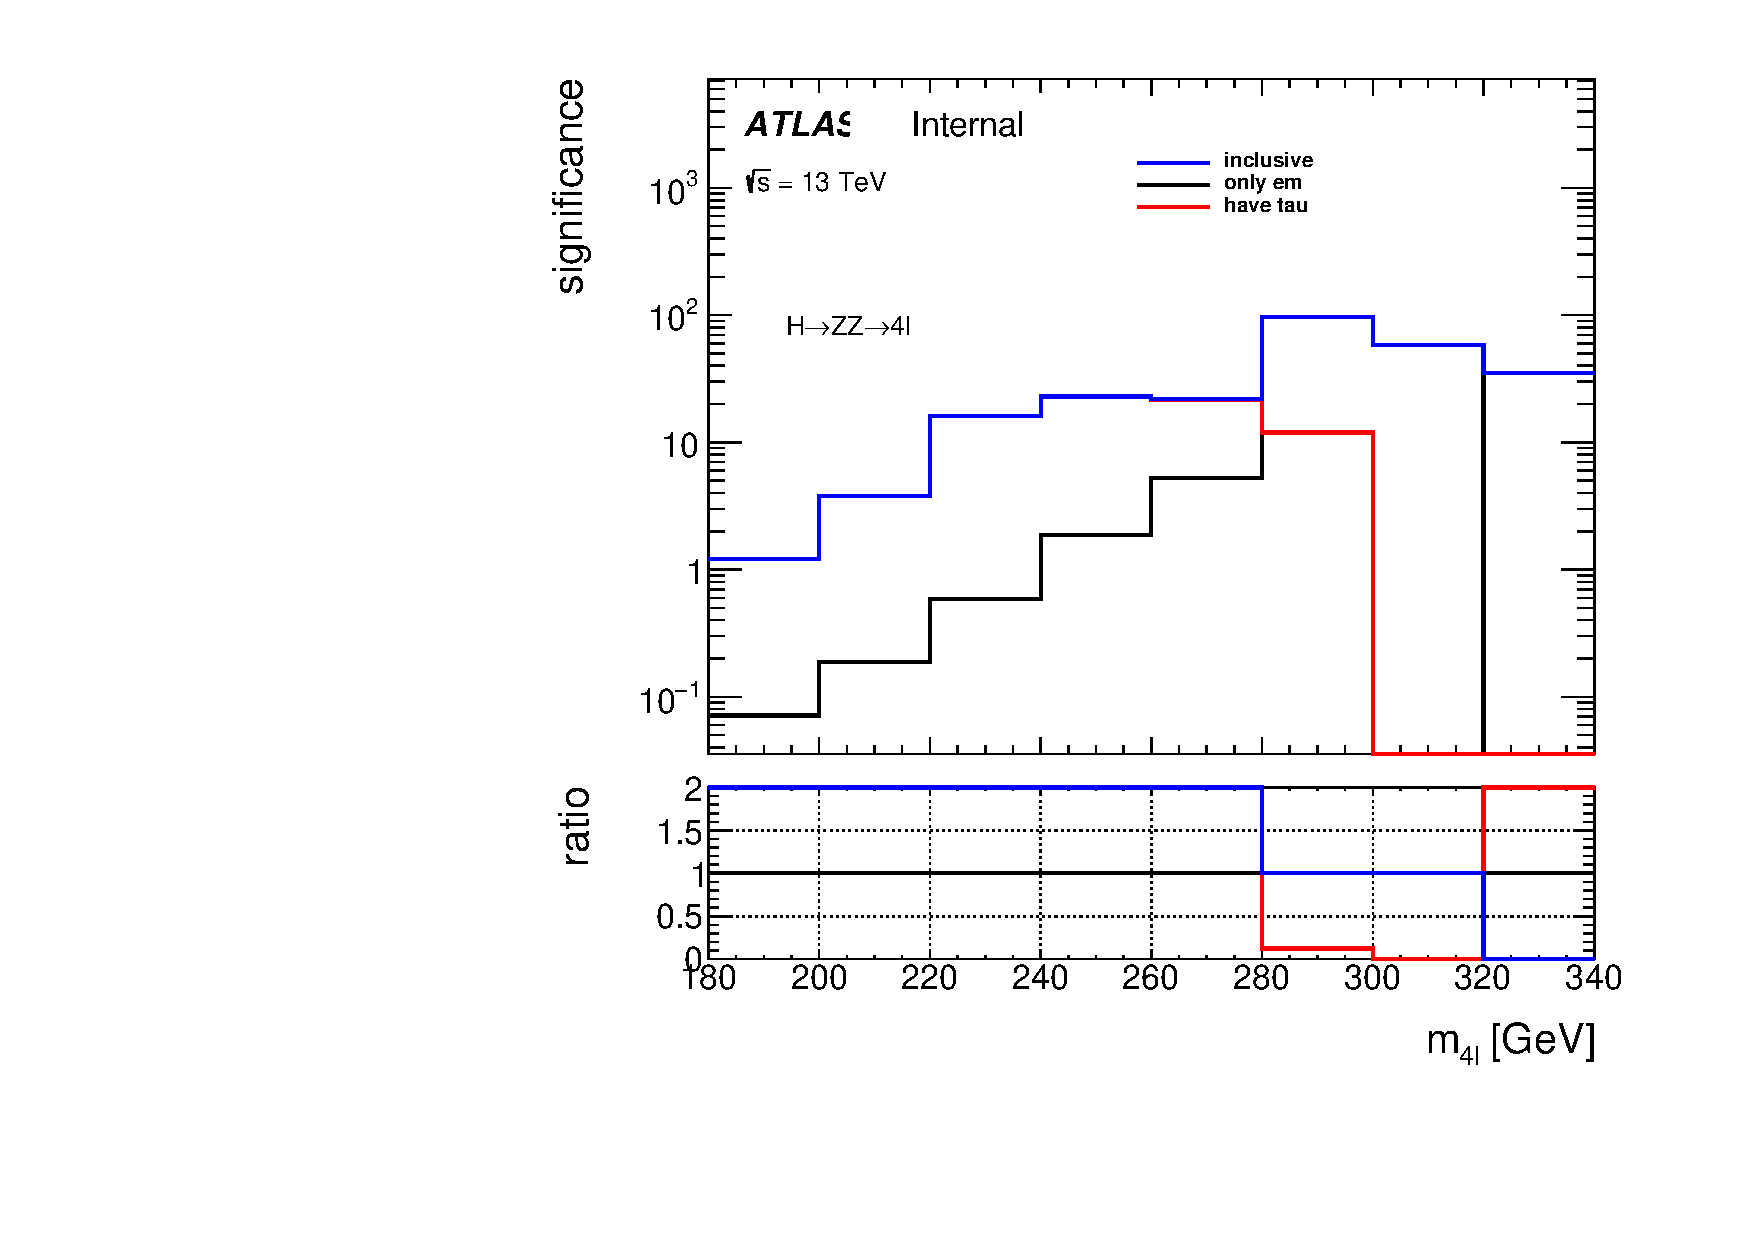
\includegraphics[width=0.48\textwidth]{figures/HMHZZ/truthTau/signf_300NW_log.pdf}}
\subfloat[]{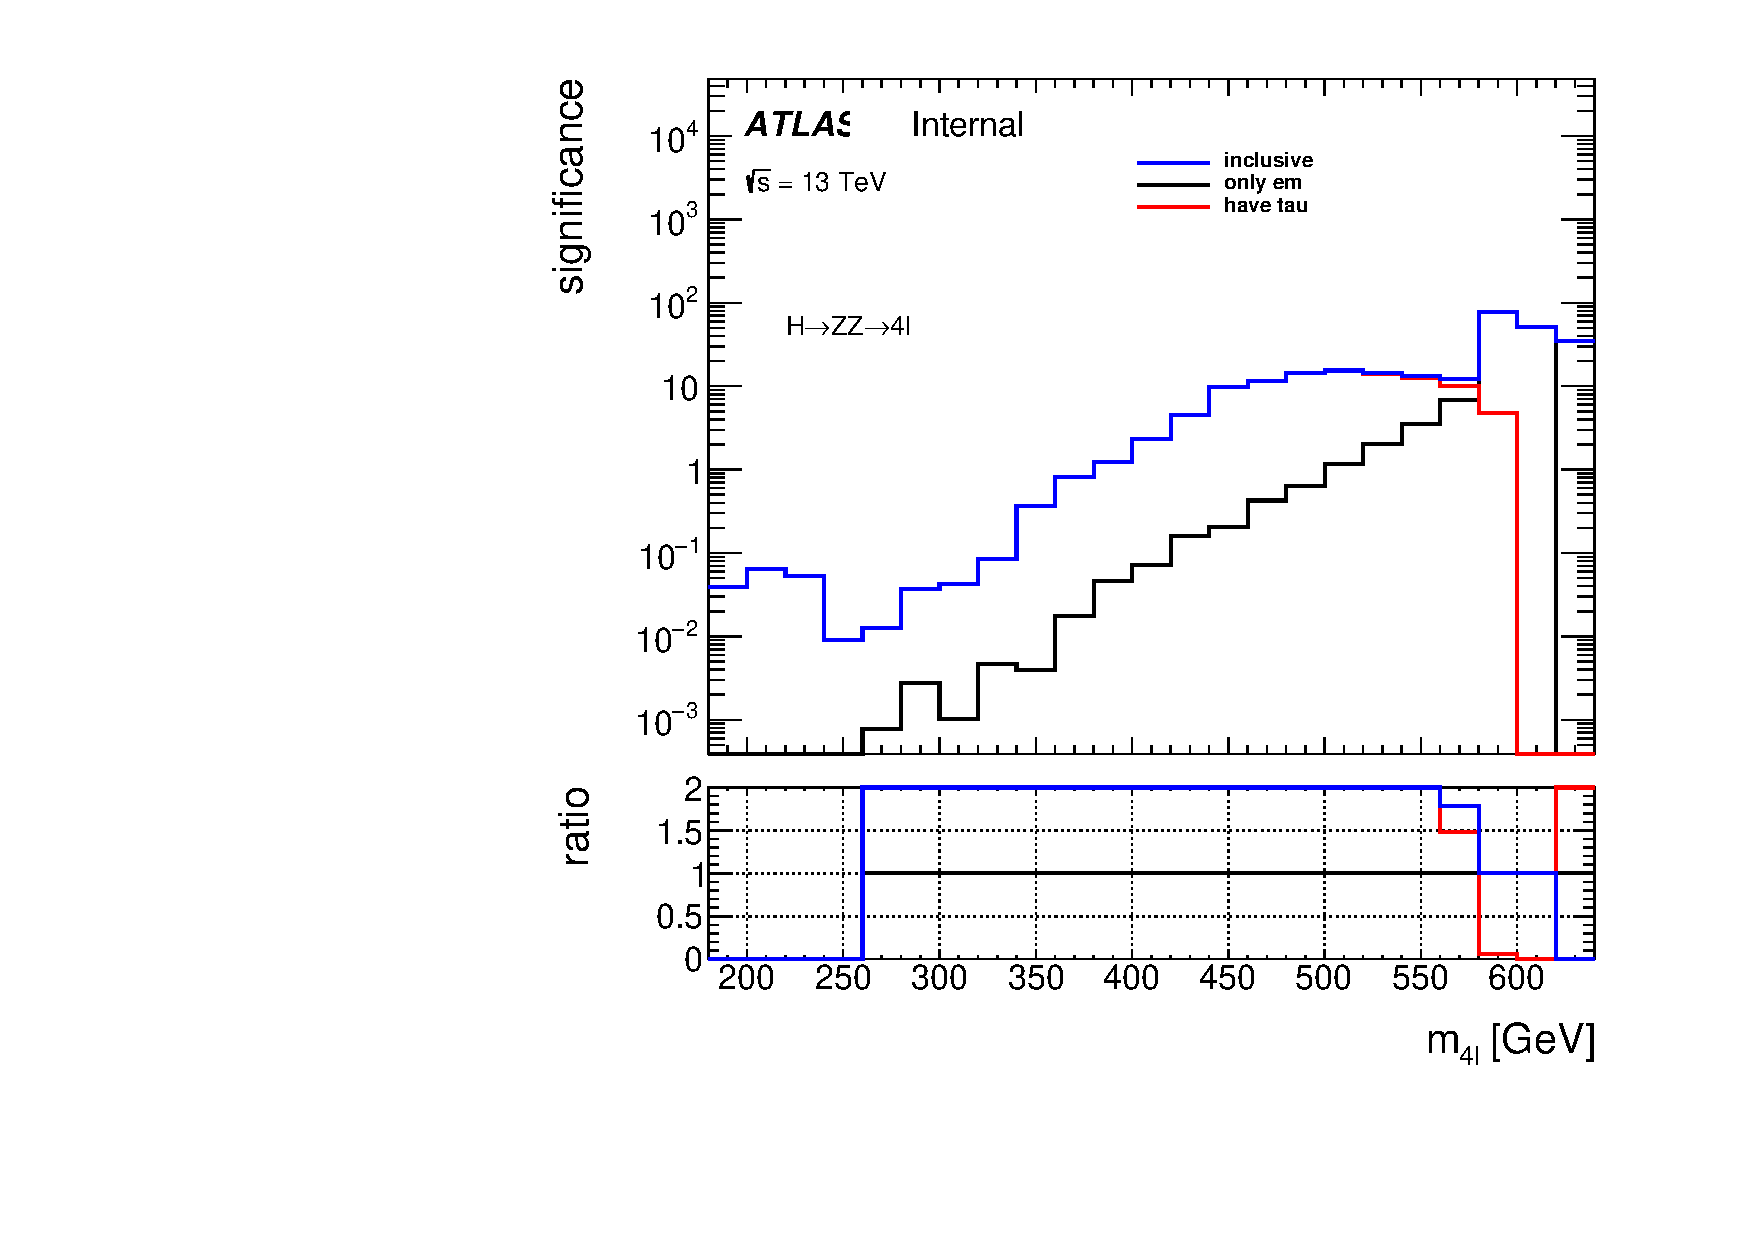
\includegraphics[width=0.48\textwidth]{figures/HMHZZ/truthTau/signf_600NW_log.pdf}}
\\
\subfloat[]{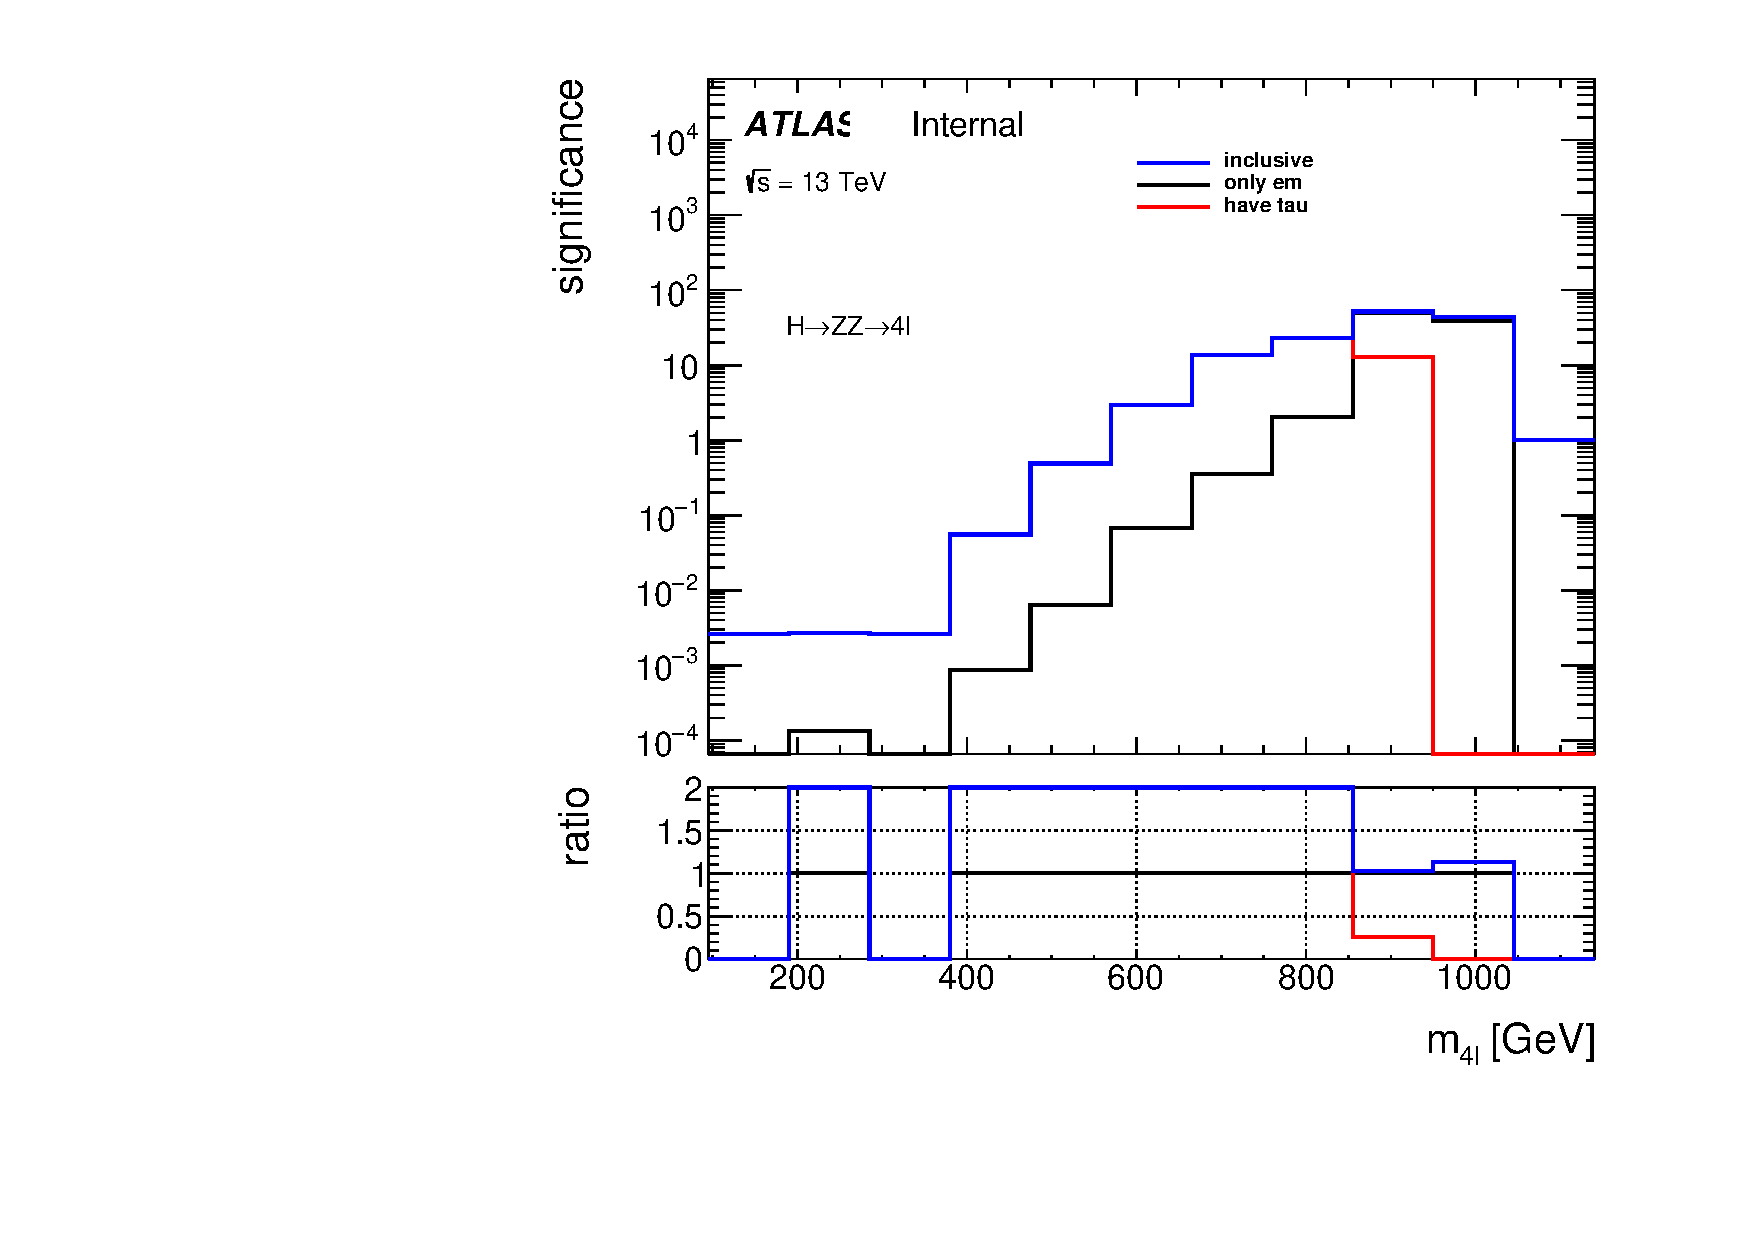
\includegraphics[width=0.48\textwidth]{figures/HMHZZ/truthTau/signf_1000NW_log.pdf}}
\subfloat[]{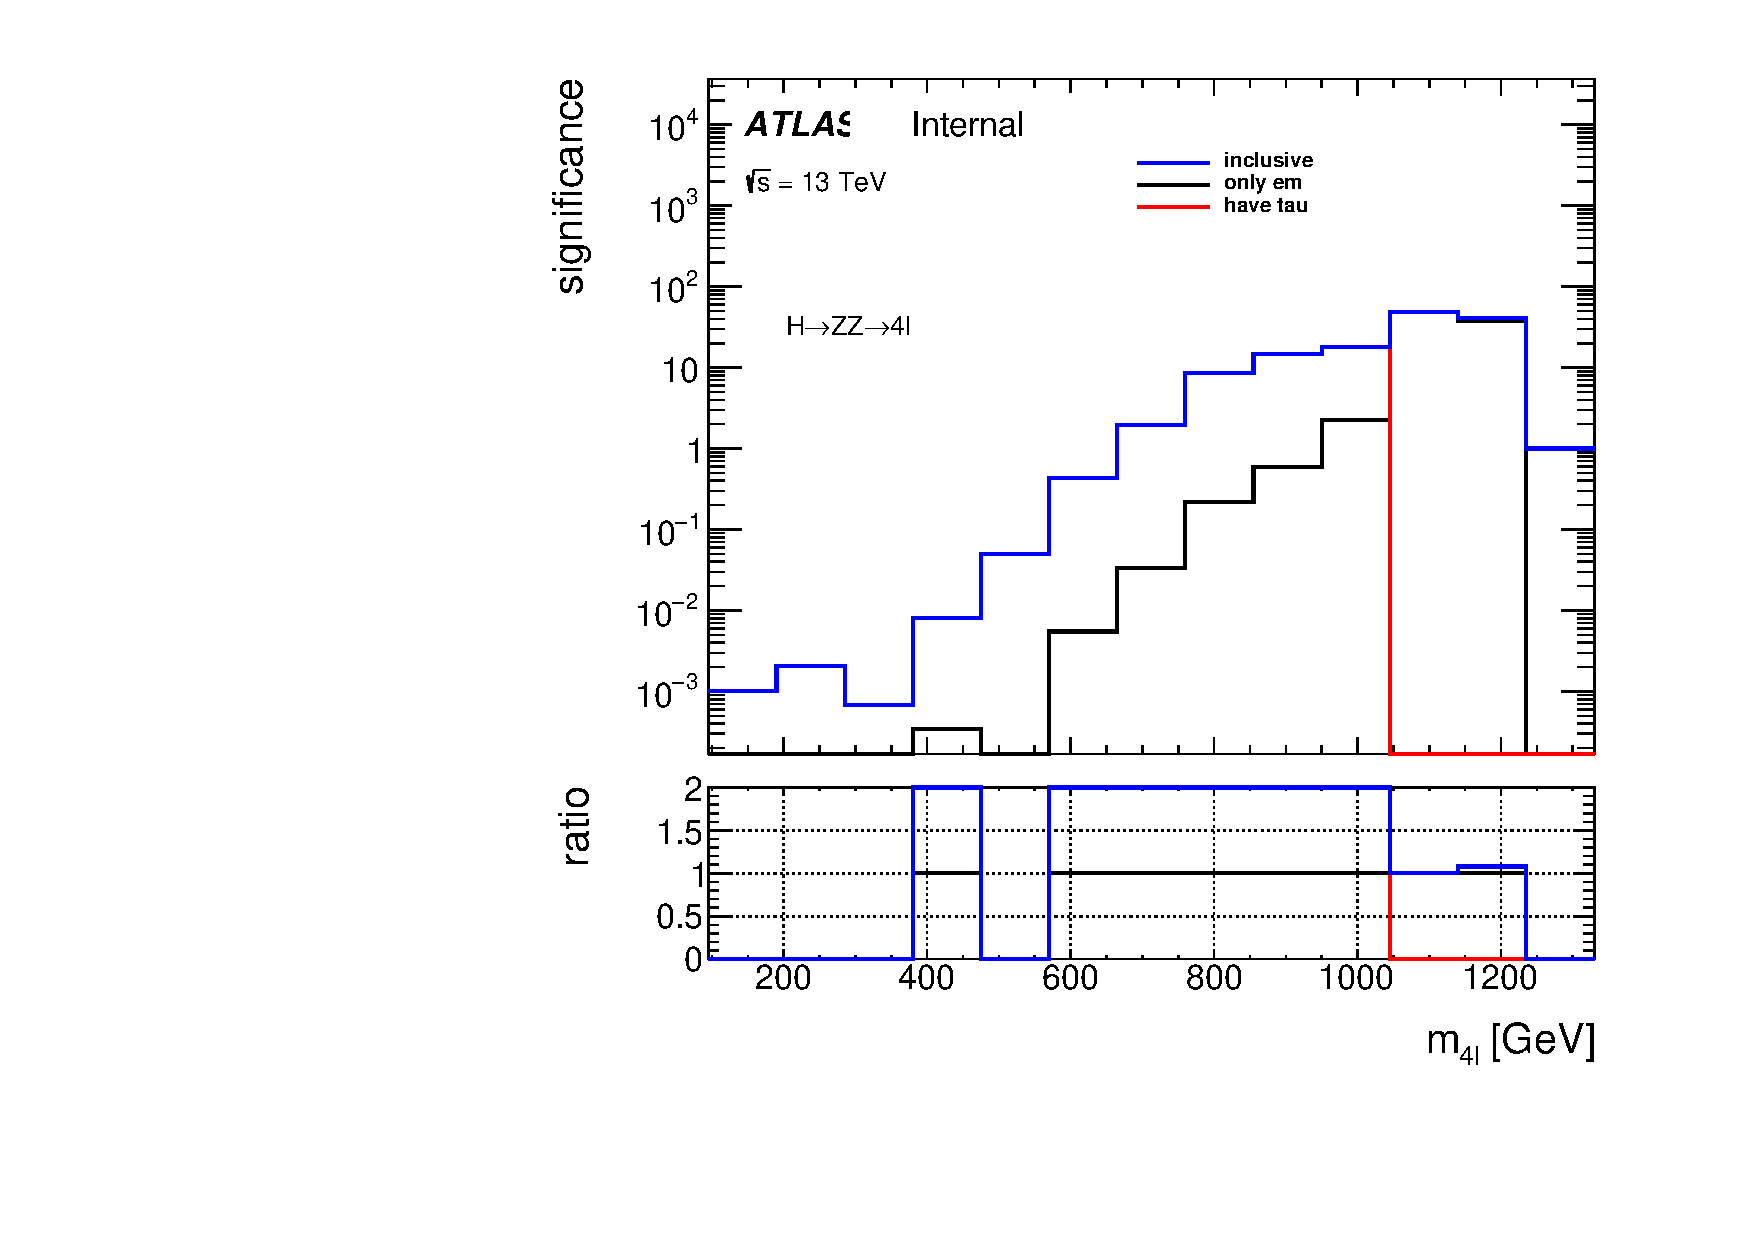
\includegraphics[width=0.48\textwidth]{figures/HMHZZ/truthTau/signf_1200NW_log.pdf}}
\caption{
Significance scan at the \mH of 
(a) 300~\gev;
(b) 600~\gev;
(c) 1000~\gev;
(d) 1200~\gev,
for events in lepton flavor channel with or without $\tau$-lepton.
}
\label{fig:tau_signif}
\end{figure}

\textbf{Using Missing Mass Calculator tool for the reconstruction of $\tau$-lepton}

As using only visible decay product of $\tau$-lepton leads to very large energy loss in reconstruction, 
an \textit{Missing Mass Calculator} (MMC) tool~\cite{elagin2011new} is applied to extract the invisible part of $\tau$ decay products.
The MMC method is a technique that can significantly improve the neutrino momentum resolutions and di-$\tau$ invariant mass,
by considering a complete reconstruction of event kinematics in two $\tau$-lepton final state.

Figure~\ref{fig:mmc_Ztt_mass} shows the mass of Z bosons reconstructed from two $\tau$s again by adding the case that di-$\tau$ mass calculated from MMC.
Better mass reconstruction can be observed than using the only visible decay products.
\begin{figure}[!htbp]
\centering
\subfloat[]{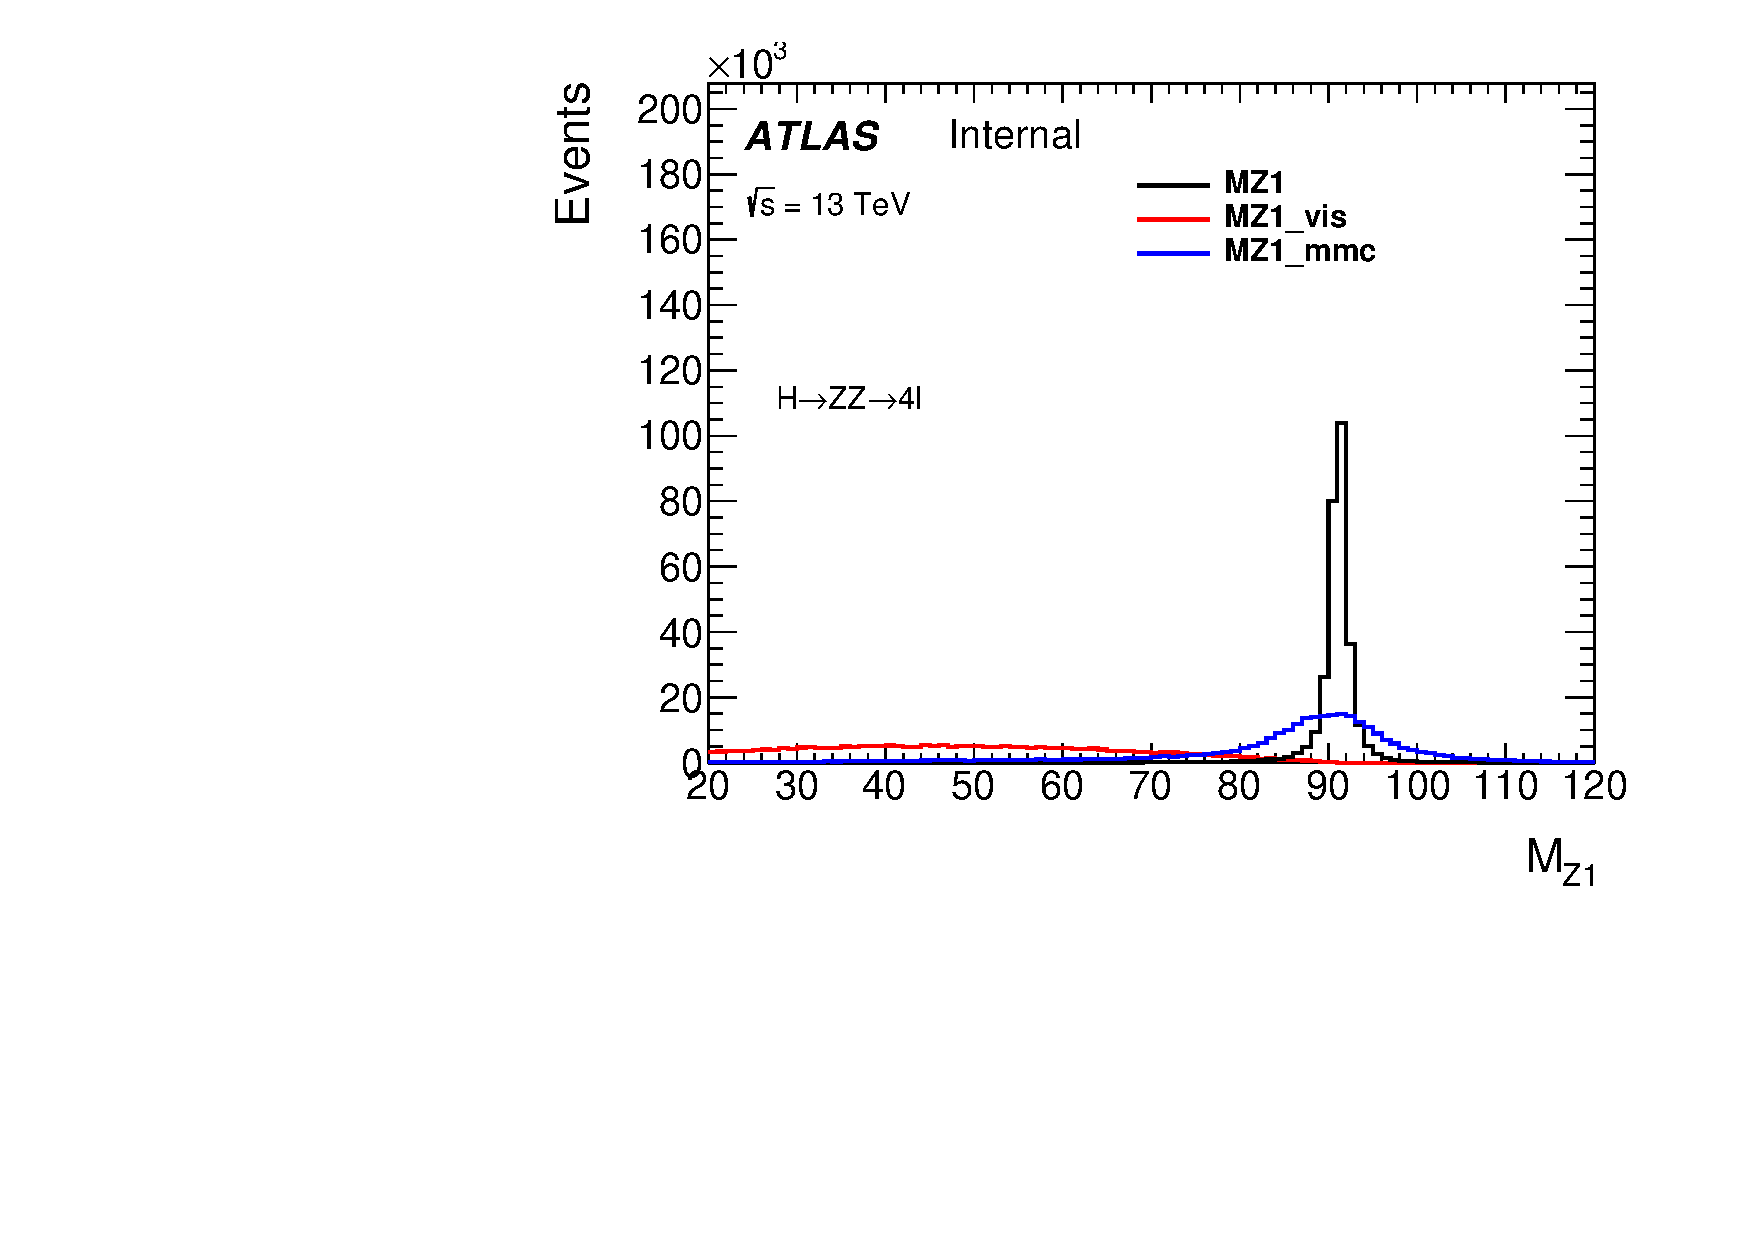
\includegraphics[width=0.48\textwidth]{figures/HMHZZ/truthTau/MZ1_300NW_linear_mmc.pdf}}
\subfloat[]{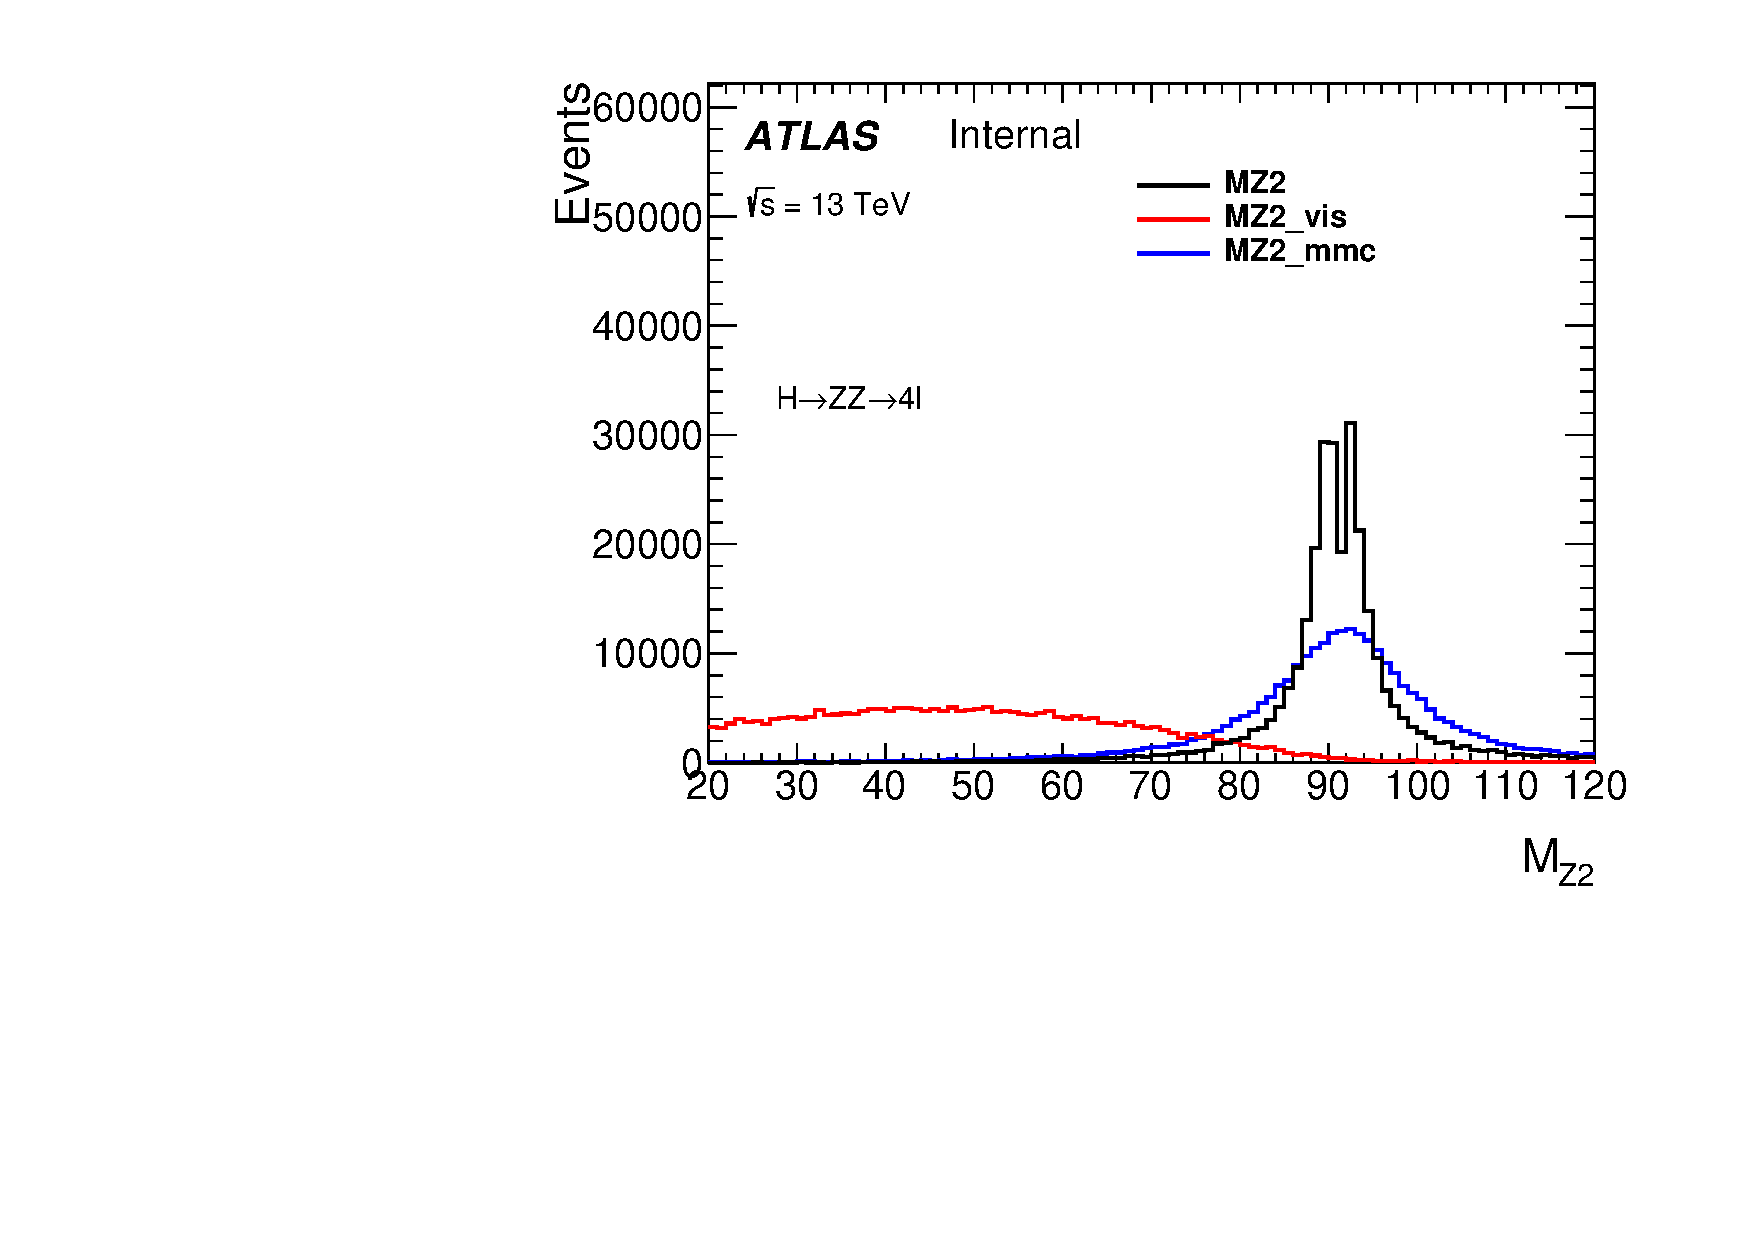
\includegraphics[width=0.48\textwidth]{figures/HMHZZ/truthTau/MZ2_300NW_linear_mmc.pdf}}
\caption{
Z(\rightarrow $\tau\tau$) boson invairant mass distribution for signal at 300~\gev~of
(a) $M_{Z1}$: the leading pairs;
(b) $M_{Z2}$: the sub-leading pairs.
The defination of leading and sub-leading pairs can be found in section~\ref{sec:hmhzz_eventsel}.
}
\label{fig:mmc_Ztt_mass}
\end{figure}

Figure~\ref{fig:mmc_4l_mass} shows the \mfl distribution after event selections for events in $2e2\mu$, 4e, and $4\mu$ channels, 
and those in $2e2\tau$ and $2\mu2\tau$ channels. 
The simulated narrow-wdith signal samples at the \mH of 300~\gev~and 1000~\gev, as well as the \qqZZ background are studied.

\begin{figure}[!htbp]
\centering
\subfloat[]{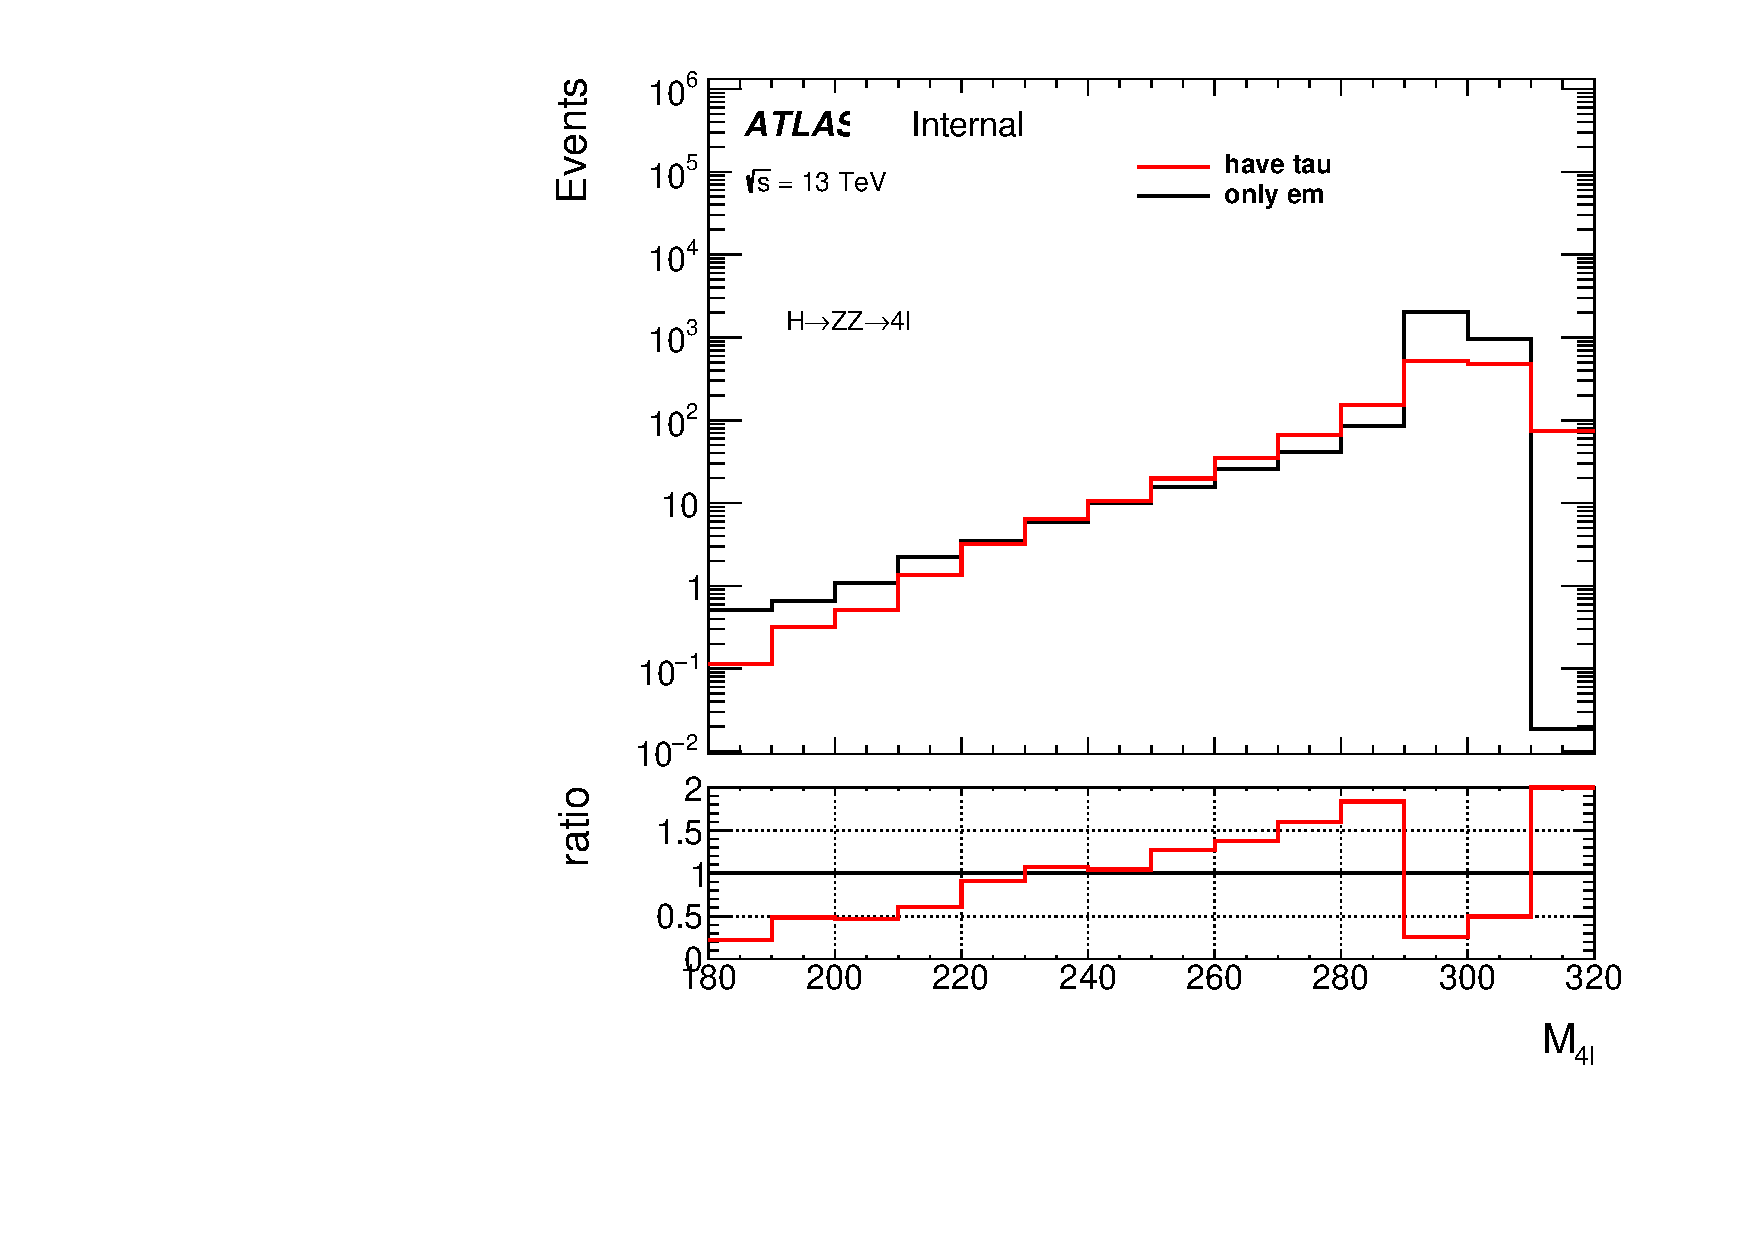
\includegraphics[width=0.33\textwidth]{figures/HMHZZ/truthTau/MZZ_emt_300NW_log_mmc.pdf}}
\subfloat[]{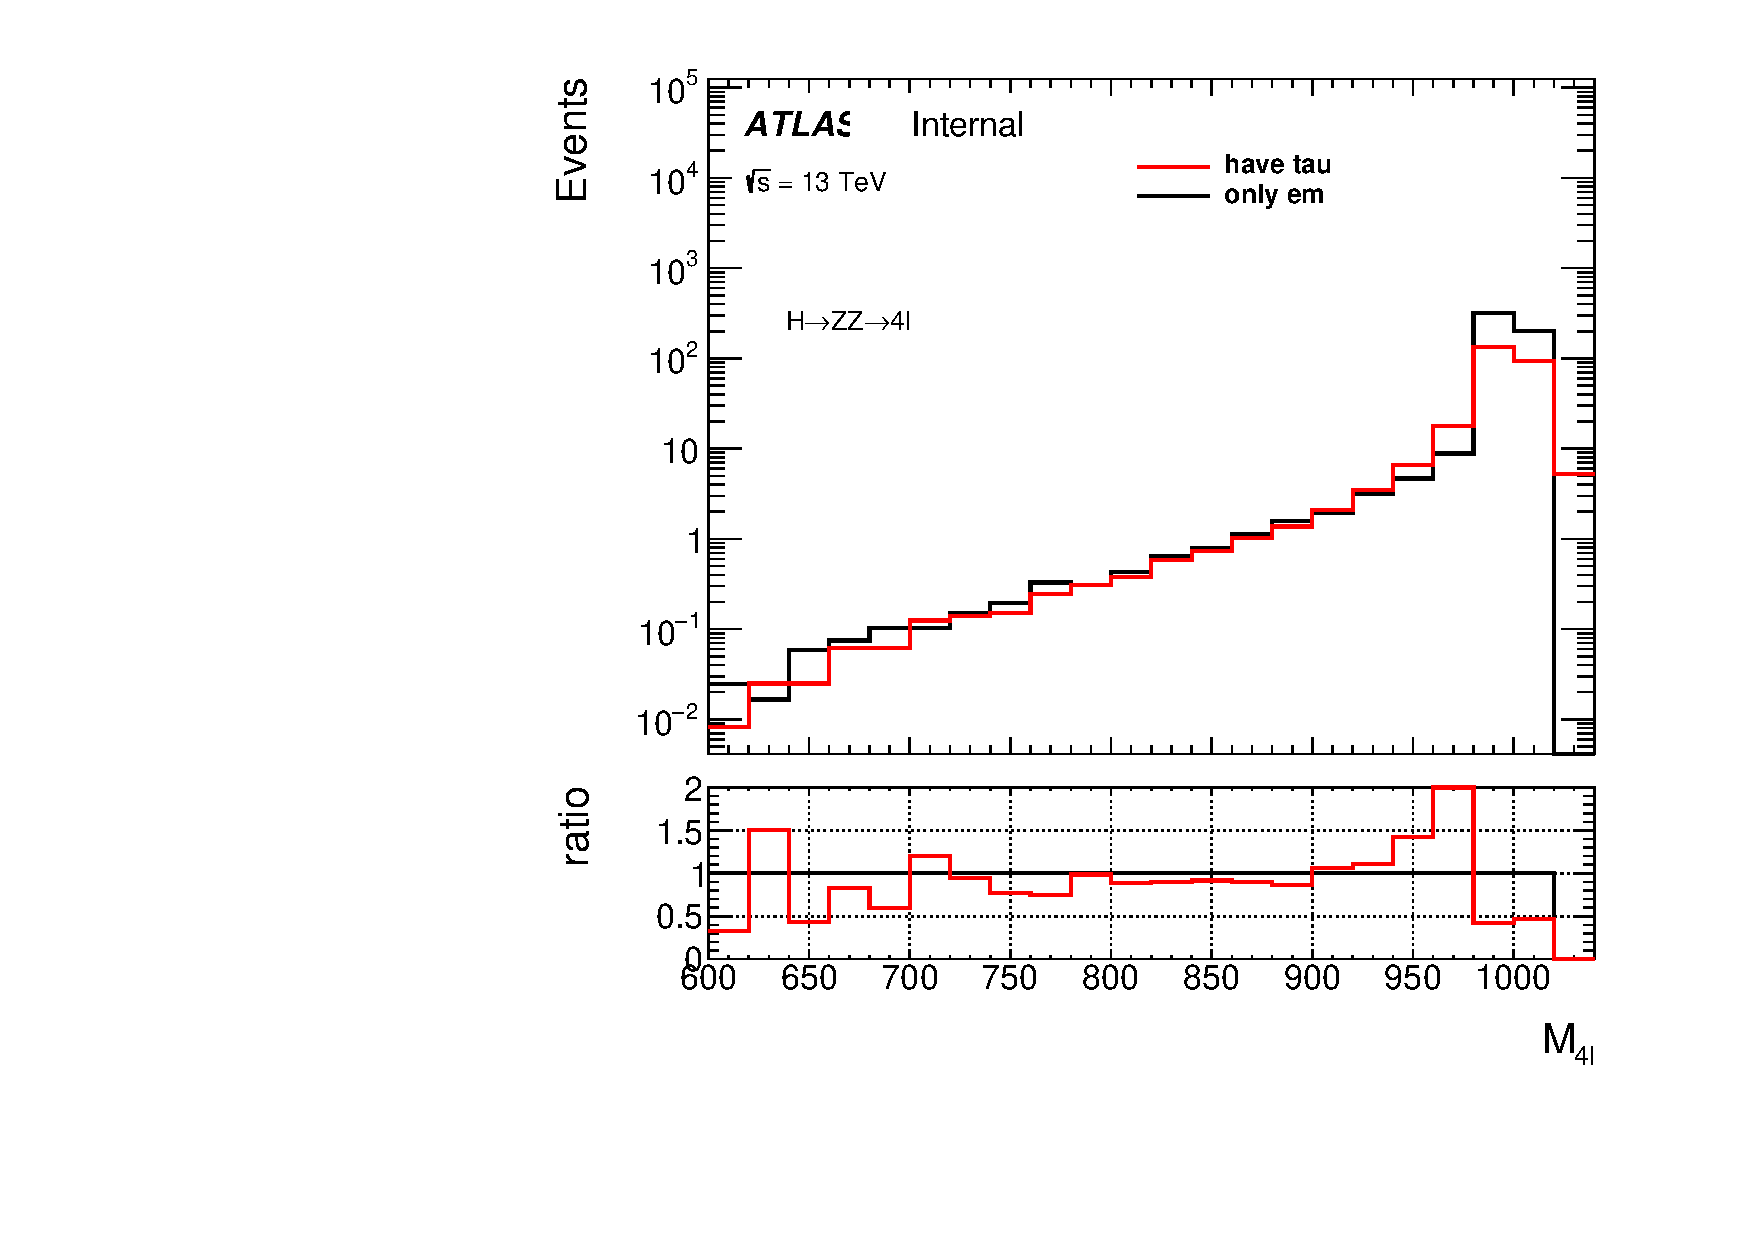
\includegraphics[width=0.33\textwidth]{figures/HMHZZ/truthTau/MZZ_emt_1000NW_log_mmc.pdf}}
\subfloat[]{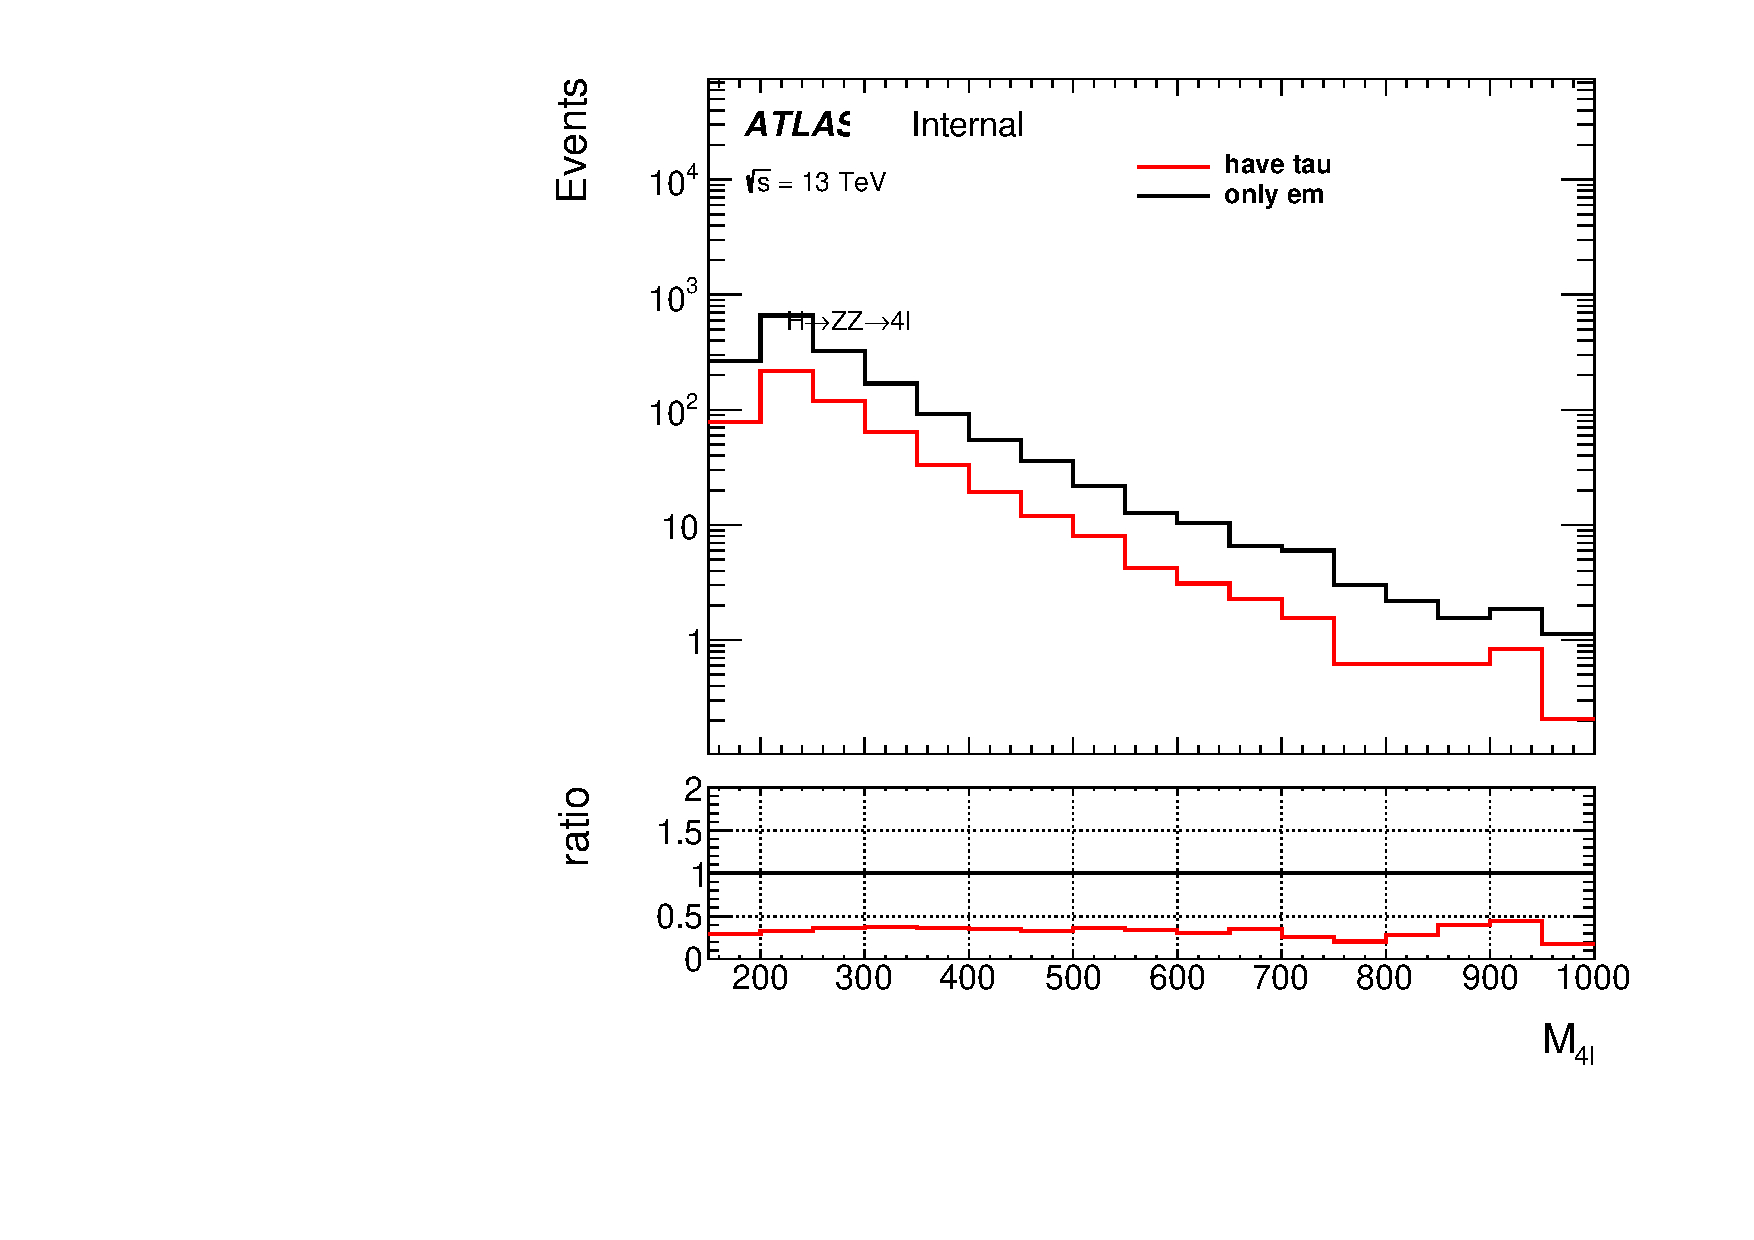
\includegraphics[width=0.33\textwidth]{figures/HMHZZ/truthTau/MZZ_emt_qqZZ_log_mmc.pdf}}
\caption{
The comaprison of \mfl distribution in the channels of
`have tau': events in $2e2\tau$ and $2\mu2\tau$ final states; `only em': events in $2e2\mu$, $4e$ and $4\mu$ final states;
for three simulated samples:
(a) NWA signal at 300~\gev;
(b) NWA signal at 1000~\gev;
(c) \qqZZ background.
}
\label{fig:mmc_4l_mass}
\end{figure}

After using MMC, the expected number of events for signal and \qqZZ background in different lepton flavor channels are shown in table~\ref{tab:yield_diffMass_mmc} by normalizing to the luminosity of 80~\ifb.

\begin{table}[htbp]
  \centering
  \caption{After using MMC, the expected number of events for signal and \qqZZ background in the lepton flavor channels with or without $\tau$-lepton.
	The event yields are normalized to the luminosity of 80~\ifb.}
  \label{tab:yield_diffMass_mmc}
  \begin{tabular}{|c|c|c|c|c|c|}
    \hline
      \multirow{2}*{Mass window} & \multirow{2}*{Channels} & \multicolumn{2}{c|}{signal} & \multicolumn{2}{c|}{\qqZZ} \\
    \cline{3-6}
      & ~ & Events & Fraction & Events & Fraction \\
    \hline
    \multirow{3}*{[250\gev, 350\gev]}  & Inclusive & 4517.2 & $100\%$  & 685.6 & $100\%$ \\
    \cline{2-6}
    ~                                  & Only e$\mu$   & 3148.2 & $69.7\%$ & 500.3 & $73.0\%$ \\
    \cline{2-6}
    ~                                  & With $\tau$  & 1369.0 & $30.3\%$ & 185.0 & $27.0\%$ \\
    \hline
    \multirow{3}*{[950\gev, 1050\gev]} & Inclusive & 785.5 & $100\%$  & 1.69 & $100\%$ \\
    \cline{2-6}
    ~                                  & Only e$\mu$   & 529.9 & $67.5\%$ & 1.26 & $74.4\%$ \\
    \cline{2-6}
    ~                                  & With $\tau$  & 255.6 & $32.5\%$ & 0.59 & $35.1\%$ \\
    \hline
  \end{tabular}
\end{table}

Figure~\ref{fig:mmc_tau_signif} shows the significance scan as a function of \mfl at two mass points: 300 and 1000~\gev, for events in lepton flavor channel with or without $\tau$-lepton. 
A profile likehood function is used for scan, and the background only considers the contribution from \qqZZ.

\begin{figure}[!htbp]
\centering
\subfloat[]{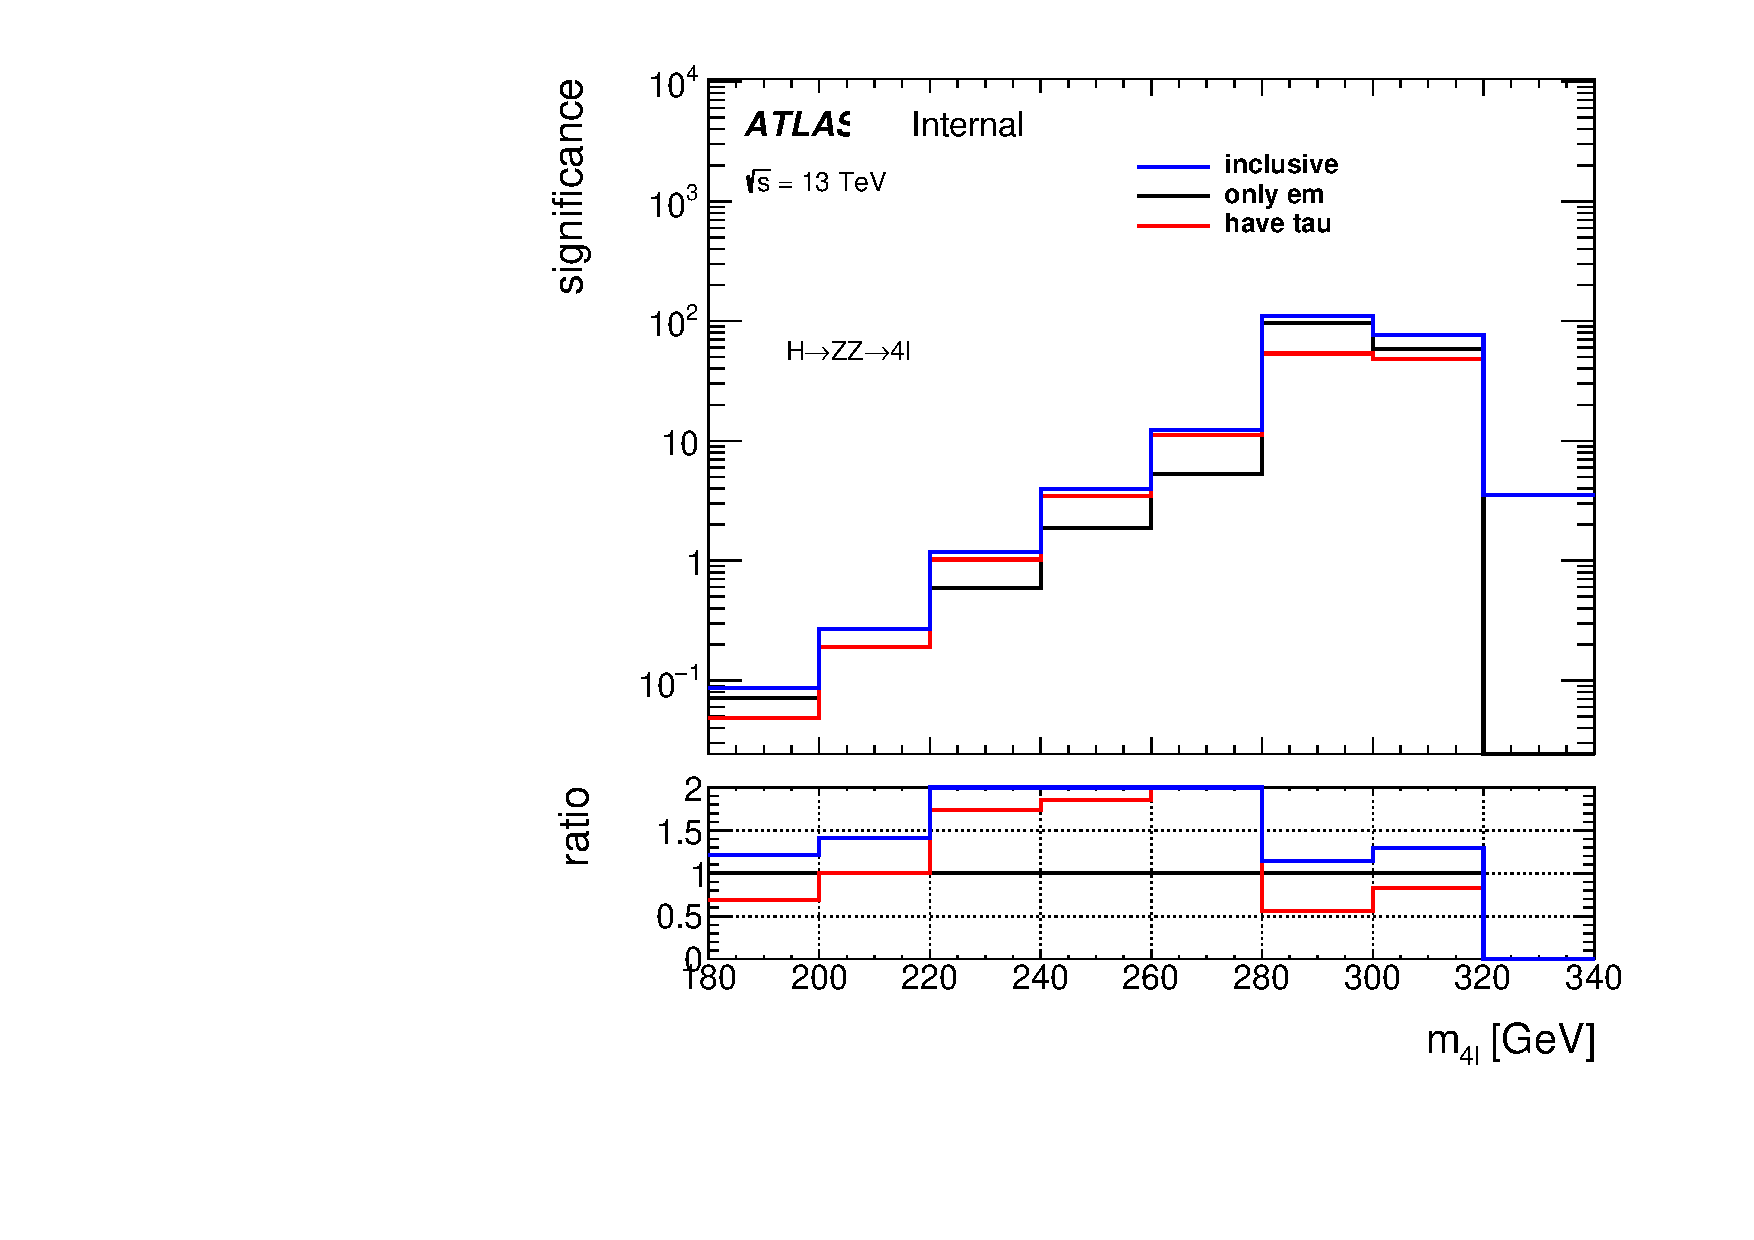
\includegraphics[width=0.48\textwidth]{figures/HMHZZ/truthTau/signf_300NW_log_mmc.pdf}}
\subfloat[]{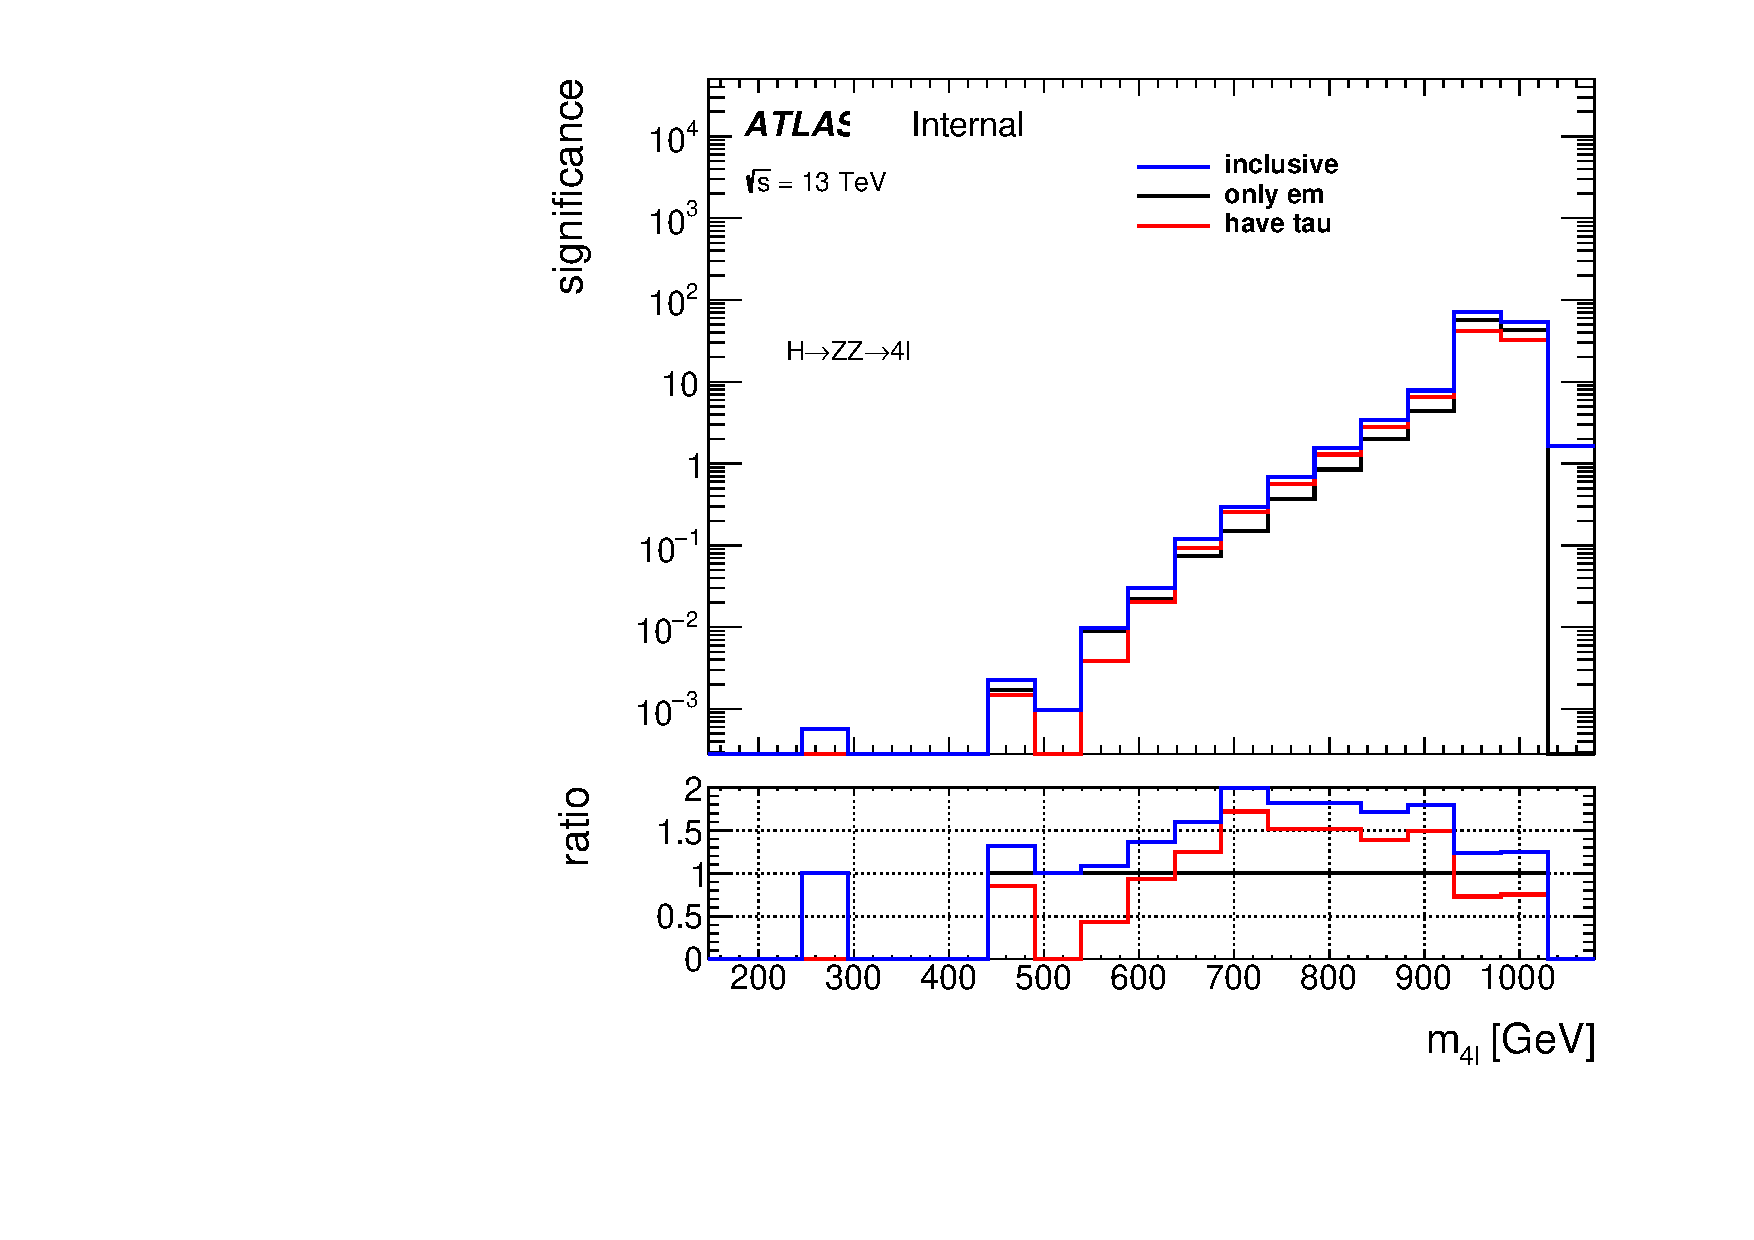
\includegraphics[width=0.48\textwidth]{figures/HMHZZ/truthTau/signf_1000NW_log_mmc.pdf}}
\caption{
Significance scan at the \mH of 
(a) 300~\gev;
(b) 1000~\gev;
for events in lepton flavor channel with or without $\tau$-lepton.
}
\label{fig:mmc_tau_signif}
\end{figure}

From the studies above in particle-level, the Missing Mass Calculator tool improves the mass reconstruction of di-$\tau$ pair significantly,
and provides a possiblity to include $\tau$-lepton into four-lepton final state analyses in the future.
But the fraction of events recontructed with $\tau$-lepton in background is still larger than the one in signal in higher mass region equal to or greater than 1000~\gev~ as shown in table~\ref{tab:yield_diffMass} and ~\ref{tab:yield_diffMass_mmc} even in particle-level.
And as the significance scan shown in figure~\ref{fig:mmc_tau_signif}, in the two \mfl bins on peak, the significance with only $\tau$-channel events is worse than other cases, which will reduce the separation power of \mfl discrinimant between signal and our backgrounds.
Considering the more complicated background components and worse reconstructed mass resolution after inviting $\tau$-lepton in reconstruction-level,
the analysis team decided not to include $\tau$-channel in this analysis.
